\subsection{Flexbox}

%
\begin{frame}
  \begin{columns}
    \column{0.45\textwidth}
      Oldalelrendezési módszer: az elemeket egy tároló belsejében jelenítik meg, egy (vagy több) tengely mentén felfűzve. A tároló (pl. \texttt{<div>} elem) \texttt{display} tulajdonságának értékei:
      \begin{description}[m]
        \item[\texttt{flex}] \hfill \\ Blokkszintű elemként
        \item[\texttt{inline-flex}] \hfill \\ Soron belüli elemként
      \end{description}
    \column{0.45\textwidth}
      \begin{exampleblock}{\textattachfile{flexbox.html}{flexbox.html}}
        \scriptsize
        \lstinputlisting[style=HTML,linerange={7-17},numbers=right,firstnumber=7]{flexbox.html}
      \end{exampleblock}
  \end{columns}
\end{frame}

%
\begin{frame}
  A tengely és bejárásának iránya a \texttt{flex-direction} tulajdonsággal változtatható:
  \begin{columns}
    \column{0.35\textwidth}
      \begin{description}[m]
        \item[\texttt{row}] \hfill \\ Vízszintes, balról jobbra (alapértelmezés)
        \item[\texttt{row-reverse}] \hfill \\ Vízszintes, jobbról balra
        \item[\texttt{column}] \hfill \\ Függőleges, fentről le
        \item[\texttt{column-reverse}] \hfill \\ Függőleges, lentről fel
      \end{description}
    \column{0.55\textwidth}
      \begin{exampleblock}{\textattachfile{flexbox.html}{flexbox.html}}
        \scriptsize
        \lstinputlisting[style=HTML,linerange={21-26},numbers=right,firstnumber=21]{flexbox.html}
      \end{exampleblock}
      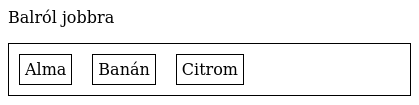
\includegraphics[width=\textwidth]{flex-direction-row.png}
  \end{columns}
\end{frame}

%
\begin{frame}
  Ha az elemek szélességeinek összege kisebb, mint a tengely hossza, akkor a \texttt{justify-content} tulajdonsággal beállítható, hová helyezzük az elemeket a tengely mentén:
  \begin{description}[m]
    \item[\texttt{flex-start}] \hfill \\ Alapértelmezés, a tengely elejére
    \item[\texttt{flex-end}] \hfill \\ A tengely végére
    \item[\texttt{center}] \hfill \\ Tengely közepére
    \item[\texttt{space-between}] \hfill \\ A tárolt elemek között egyforma méretű helyet hagy
    \item[\texttt{space-around}] \hfill \\ Minden tárolt elem mindkét oldalán azonos helyet hagy, a szomszédos üres részeket nem vonja össze
  \end{description}
\end{frame}

%
\begin{frame}
  \begin{exampleblock}{\textattachfile{flexbox.html}{flexbox.html}}
    \scriptsize
    \lstinputlisting[style=HTML,linerange={57-68},numbers=left,firstnumber=57]{flexbox.html}
  \end{exampleblock}
\end{frame}

%
\begin{frame}
  \begin{center}
    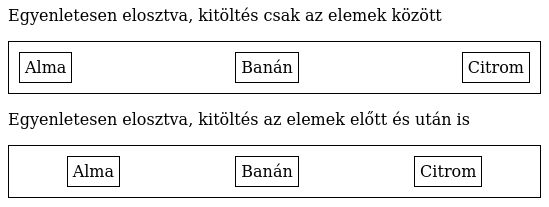
\includegraphics[width=.75\textwidth]{justify-content-space-between.png}
  \end{center}
\end{frame}

%
\begin{frame}
  Ha az elemek nem férnek el egymás mellett a tengely mentén, akkor a \texttt{flex-wrap} tulajdonságtól függ, mi történik:
  \begin{description}[m]
    \item[\texttt{nowrap}] \hfill \\ Alapértelmezés, a tárolt elemek kilógnak / nem jelennek meg
    \item[\texttt{wrap}] \hfill \\ További párhuzamos tengelyeket hoz létre
    \item[\texttt{wrap-reverse}] \hfill \\ Mint \texttt{wrap}, de a tengelyek sorrendje fordított
  \end{description}
  \vfill
  A \texttt{flex-direction} és \texttt{flex-wrap} tulajdonságok egy összetett tulajdonságon keresztül is állíthatók: \\
  \texttt{flex-flow: \emph{flex-direction flex-wrap}}
\end{frame}

%
\begin{frame}
  \begin{exampleblock}{\textattachfile{flexbox.html}{flexbox.html}}
    \scriptsize
    \lstinputlisting[style=HTML,linerange={107-109},numbers=left,firstnumber=107]{flexbox.html}
    \lstinputlisting[style=HTML,linerange={116-117},numbers=left,firstnumber=116]{flexbox.html}
  \end{exampleblock}
  \begin{columns}
    \column{0.55\textwidth}
      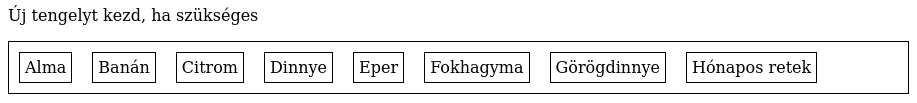
\includegraphics[width=\textwidth]{flex-wrap1.png}
    \column{0.4\textwidth}
      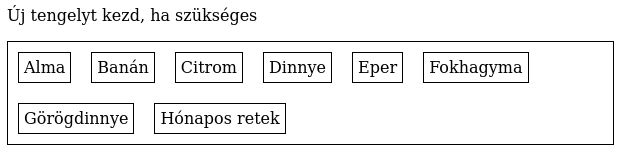
\includegraphics[width=\textwidth]{flex-wrap2.png}
  \end{columns}
\end{frame}

%
\begin{frame}
  Az elemeknek a tengelyre merőleges irányban történő méretezését / elhelyezését befolyásolja az \texttt{align-items} tulajdonság:
  \begin{description}[m]
    \item[\texttt{stretch}] \hfill \\ Kinyújtás a tároló széléig
    \item[\texttt{flex-start}] \hfill \\ Az elemeket balra / felfelé igazítja
    \item[\texttt{flex-end}] \hfill \\ Jobbra / lefelé igazít
    \item[\texttt{center}] \hfill \\ Középre igazít
    \item[\texttt{baseline}] \hfill \\ Az alapvonalhoz igazít
  \end{description}
\end{frame}

%
\begin{frame}
  A tárolóra beállított \texttt{align-items} minden elem megjelenítését befolyásolja, de ez az elemek \texttt{align-self} tulajdonságán keresztül egyedileg felülírható.
  \vfill
  \begin{columns}
    \column{0.65\textwidth}
      \begin{exampleblock}{\textattachfile{flexbox.html}{flexbox.html}}
        \scriptsize
        \lstinputlisting[style=HTML,linerange={99-106},numbers=left,firstnumber=99]{flexbox.html}
      \end{exampleblock}
    \column{0.3\textwidth}
      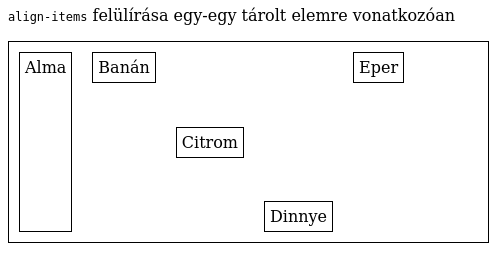
\includegraphics[width=\textwidth]{align-self.png}
  \end{columns}
\end{frame}

%
\begin{frame}
  Az \texttt{align-content} a tengelyek tárolón belüli elhelyezését befolyásolja. Értékei ugyanazok, mint \texttt{align-items}-nek. Akkor látványos a hatása, ha több tengelyre van szükség az elemek elhelyezéséhez.
  \vfill
  Ha az elemek HTML-ben specifikált sorrendjétől eltérő sorrendben szeretnénk azokat a tengelyre felfűzni, minden elemhez megadhatjuk a kívánt pozíciót az \texttt{order} tulajdonság értékeként.
  \vfill
  \begin{columns}
    \column{0.65\textwidth}
      \begin{exampleblock}{\textattachfile{flexbox.html}{flexbox.html}}
        \scriptsize
        \lstinputlisting[style=HTML,linerange={151-156},numbers=left,firstnumber=151]{flexbox.html}
      \end{exampleblock}
    \column{0.3\textwidth}
      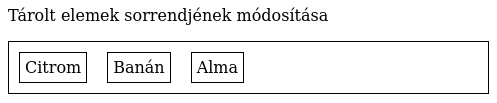
\includegraphics[width=\textwidth]{order.png}
  \end{columns}
\end{frame}

%
\begin{frame}
  Az elemek között arányosan szétosztható a konténer területe, azok \texttt{flex} tulajdonságainak beállításával: \texttt{flex: \emph{flex-grow flex-shrink flex-basis}}
  \vfill
  \begin{columns}
    \column{0.6\textwidth}
      \begin{exampleblock}{\textattachfile{flexbox.html}{flexbox.html}}
        \scriptsize
        \lstinputlisting[style=HTML,linerange={163-168},numbers=left,firstnumber=163]{flexbox.html}
      \end{exampleblock}
    \column{0.35\textwidth}
      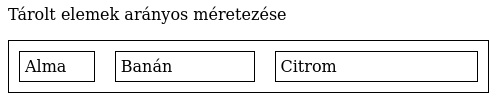
\includegraphics[width=\textwidth]{flex.png}
  \end{columns}
  \vfill
  Beállítások hatása gyakorlatban kipróbálható: \textattachfile{flextest.html}{flextest.html}
\end{frame}
